% \chapter{ICM} % Lecture 11/03/2026

% \section{Introduction}

% % missing STRUCTURE FORMATION: DARK MATTER HALOS

% \subsection{Galaxy Clusters}

% Galaxy clusters are composed of galaxies, dark matter, and hot gas. They are the most massive structures in the universe, with a mass $M = 10^{14} - 10^{15} M_\odot$ and a radius $R = 1-5 Mpc$.

% Form from the highest density peak of the initial matter density field, Preferentially located at the knots of the Large Scale Structure (LSS).

% Galaxy clusters are multi-component systems:

% Galaxies and stars (~5\%), ICM (~15\%), DM (~80\%)

% Allow to detect clusters at different wavelengths: X-rays, radio, optical, infrared, ultraviolet, gamma-rays.

% Perfect astrophysical laboratory to study: galaxy evolution, gas and plasma astrophysics

% \subsubsection{Cluster boundary}

% The boundary of the cluster is not a well-defined quanrity: clusters are not closed spheres, however it is convenient to define a cluster as the mass within a certain radius, corresponding to a fixed overdensity $\Delta$.

% $\Delta$ is defined as the overdensity with respect to the mean or the critical density of the Universe at the cluster redshift.

% $$
% M_{\Delta} = \dfrac{4\pi}{3} r^3_{\Delta} \rho_{m/cr} \Delta
% $$

% %todo: check if true
% where $\rho_{m/cr}$ is the mean or critical density of the Universe at the cluster redshift.

% The edge of the cluster can be defined by the orbital dynamics of the matter within the cluster: the \textbf{Splashback radius} is the radius of the cluster at which the expansion of the universe is equal to the gravitational pull of the cluster.

% The splashback radius represents the location of the first orbital "turnaround", i.e. the maximum distance a particle reaches after its first passage through the cluster. At the location of the Splashback radius is expected a rapid decline of the density profile.

% \begin{figure}[H]
%     \centering
%     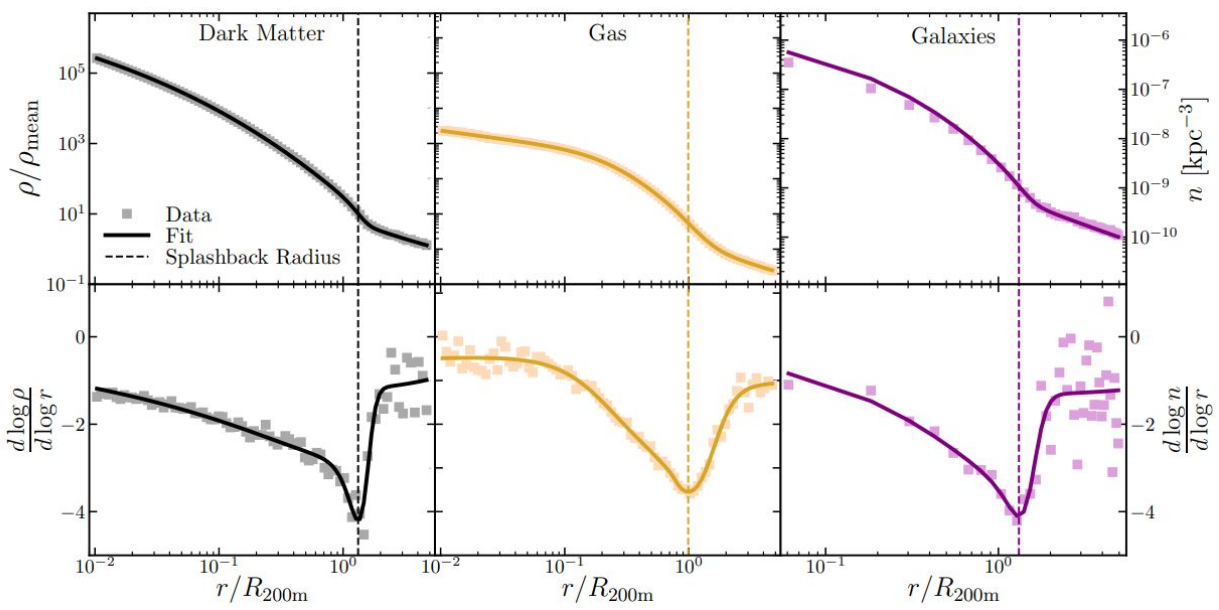
\includegraphics[width=0.6\textwidth]{assets/splashback.png}
%     \caption{DM, gas and galaxy density profiles and splashback radius from TNG hydrosim \cite{ONeil2020}.}
% \end{figure}

% \section{The intracluster medium}

% \begin{itemize}
%     \item Hot (107 - 10° K), optically thin plasma, that permeates the space between galaxies within a GC
%     \item Result of the gas infall into the dark matter halo
%     \item The gas is heated primarily through accretion shocks and adiabatic compression during the hierarchical assembly of the cluster
%     \item AGN feedback and sloshing of the ICM plasma during mergers with subclusters prevent the central ICM from cooling
%     \item Fossil record of the chemical enrichment of the Universe: the deep gravitational potential wells of clusters lock metals produced by member galaxies
%     \item Density: $\sim 10^{-3} - 10^{-1} \text{particle/cm}^3$ 
%     \item Composition: fully ionized plasma; mostly H, He with metallic traces (Fe, O, Ne, Si)
%     \item Weak but pervasive magnetic field: $\sim 0.1 \text{ to } 10 \mu\text{G}$ influencing particle transport. The field varies on scales     from $0.1 \text{ to } 10 \text{ kpc}$.
%     \item Emission primarly via X-ray:
%     \begin{itemize}
%         \item Free-free: Thermal bremsstrahlung radiation $\sim 90\%$ of the luminosity (continuum)
%         \item Free-bound: recombination (continuum)
%         \item Bound-bound: de-excitation radiation (line emission)
%     \end{itemize}
% \end{itemize}

% \subsubsection{X-Ray spectrum}

% Bremsstrahlung spectrum:
% \begin{itemize}
%     \item Bremsstrahlung X-ray emissivity:
%     $$
%     \epsilon_\nu \equiv \dfrac{\mathrm{d}L}{\mathrm{d}V\mathrm{d}\nu} \propto n_e^2 g(\nu, T) T^{-1/2} \exp(-h\nu / k_B T)
%     $$
%     \item Proportional to the square of the gas density
%     \item The overall normalization scales as $\propto T^{-0.5}$
%     \item Exponential thermal cut-off at the electron's kinetic energy ($k_B T$)
%     \begin{itemize}
%         \item The location of the cut-off provides strong constraints on the ICM temperature
%     \end{itemize}
% \end{itemize}

% The observed spectrum is a combination of the bremsstrahlung spectrum and recombination/emission lines:

% \begin{itemize}
%     \item Recombination lines: "edges" in the lower temperature spectra (e.g. 1 keV line around 0.5--1 keV)
%     \begin{itemize}
%         \item Above ${\sim}\,6$ keV the cross-section for electron capture drops significantly and the "edges" get smeared out
%     \end{itemize}
%     \item Emission lines:
%     \begin{itemize}
%         \item Strength of the line depends on temperature (e.g. Fe K-$\alpha$ @ $k \sim 6.7$ eV)
%         \item Soft X-ray lines (0.5--2 keV): due to elements like O, Ne, Mg $\rightarrow$ present only if the metals are not fully ionized ($<6$ keV)
%         \item Most prominent signature of the metal enrichment is the Fe K-line complex at 6.7 keV
%         \item Fe-K is the only accessible line at high-$z$ $\rightarrow$ only means to determine cluster redshift from X-ray data
%         \item Iron L-shell Complex (at ${\sim}\,1$ keV): caused by hundreds of overlapping emission lines from partially ionized Fe atoms ($\text{Fe}^{16}$ to $\text{Fe}^{23}$) 
%         \item ``Soft'' elements (0.5--3.0 keV) lines: useful diagnostic for star formation history
%     \end{itemize}
% \end{itemize}

% \begin{observationblock}[Spectral fitting]
%     In modern X-ray astronomy (using satellites like \bfit{Chandra} or \bfit{XMM-Newton}), the spectral resolution isn't always high enough to see the individual lines.
    
%     Observed spectra are fitted to plasma radiation codes which includes all the known emission processes.
% \end{observationblock}

% \subsubsection{Temperature profile}

% By fitting observed X-ray spectra measured at different radii with tabulated spectral emission convolved with the instrument response, is it possible to derive the ICM temperature profile.

% \noindent
% \begin{minipage}[t]{0.65\textwidth}
% \begin{itemize}
%     \item Expected cooling curve for a gas in hydrostatic equilibrium
%     \item At large radii, $R > 0.2\, R_{200}$, the normalized profile looks self-similar
%     \begin{itemize}
%         \item The same gravity-driven physics shape all clusters
%     \end{itemize}
%     \item Some profiles show a significant drop in temperature toward the core (\textbf{Cool Core}) while other profiles are $\sim$flat (\textbf{Non-Cool Core})
%     \item To accommodate the variety of temperature profiles, Vikhlinin et al. 2006 introduced the parametric model:
%     $$
%     T_{3D} = T_0 \dfrac{(r/r_t)^{-a}}{[1 + (r/r_t)^b]^{c/b}} \cdot \dfrac{x + T_{min}/T_0}{x + 1}
%     $$
% \end{itemize}
% \end{minipage}%
% \hfill
% \begin{minipage}[t]{0.3\textwidth}
%     \centering
%     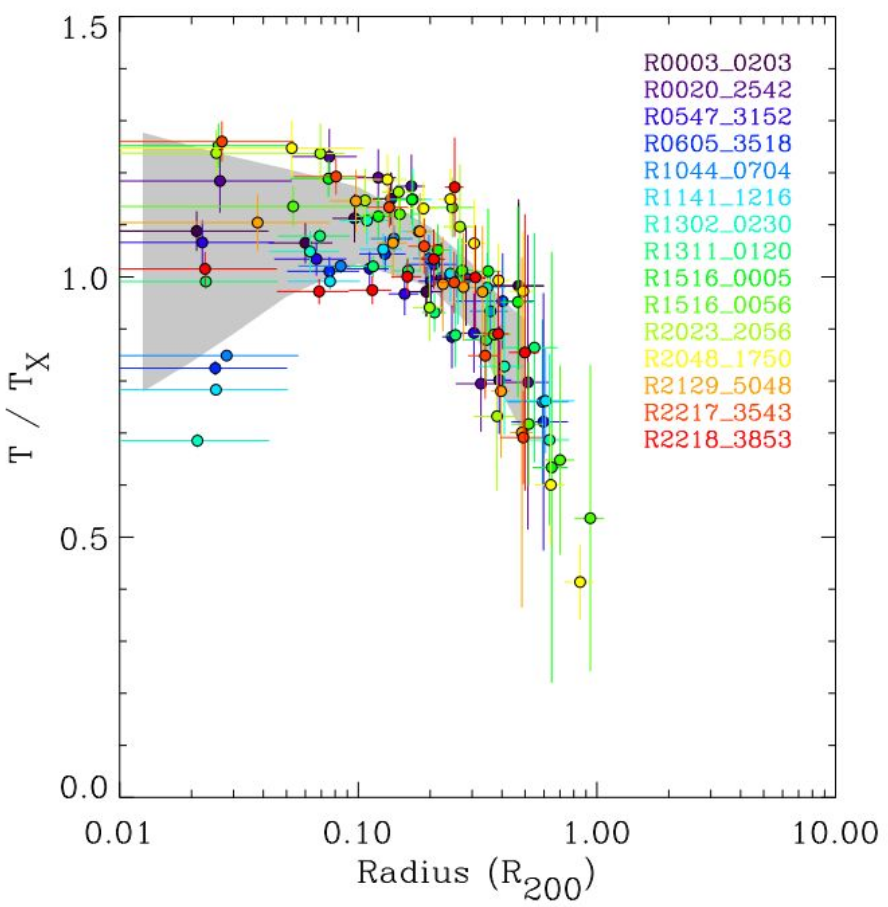
\includegraphics[width=\textwidth]{assets/gc-temp.png}
%     \captionof{figure}{Temperature profile from XMM-Newton observations \cite{Pratt2006}.}
% \end{minipage}

% \subsubsection{Metallicity profile}

% The metallicity profile shows a sharp rise toward the center ($R/R_{500} < 0.2$), reaching $\sim$solar  value in the inner core. The peak is driven by the metal production of the central galaxy.

% At large radii ($R/R_{500} > 0.3$), the profiles flatten out to a constant value $A\sim0.3$. This value is consistent across different clusters and extends so far out in radius that it suggests early enrichment (z = 2-3) of the medium.

% The evolution of the Fe abundance with redshift confirm early enrichment of the medium 

% %todo: missing last slide about metallicity profile

% \subsubsection{Gas Density profile}

% The $\beta$-model is a simple and widely used approximation for the gas density profile. Assuming an isothermal sphere, equating the Jeans and HE mass estimates leads to the definition of the $\beta$ parameter:

% $$
% M(r) = -\dfrac{\sigma_r^2 r}{G} \left[ \dfrac{d \ln \rho}{d \ln r} \right]
% \qquad
% M(r) = -\dfrac{kT r}{G \mu m_p} \left[ \dfrac{d \ln \rho_g}{d \ln r} \right]
% $$

% $$
% \beta = \dfrac{\sigma_r^2 \mu m_p}{kT}
% $$

% If the gas distribution follows the matter distribution, and the latter follows an isothermal sphere model we get:

% $$
% \dfrac{\rho_g}{\rho_{g0}} = \left( \dfrac{\rho}{\rho_0} \right)^\beta
% \qquad
% \rho = \rho_0 \left( 1 + \left( \dfrac{r}{r_c} \right)^2 \right)^{-3/2}
% \qquad
% \rho_g = \rho_{g0} \left( 1 + \left( \dfrac{r}{r_c} \right)^2 \right)^{-3\beta/2}
% $$

% Fit to data finds $\beta \sim 2/3$ , but the $\beta$-model provides a poor fit to distributed systems.

% Vikhlinin et al 2006 model:

% The $\beta$-model is a poor description of the actual density profile; The shape of cluster density profiles is affected by the individual evolution history of the cluster (e.g. merging, AGN feedbacks)

% Vikhlinin introduced in 2006 a parametric model to account for the variegate cluster population:

% $$
% n_p n_e = n_0^2 \dfrac{(r/r_c)^{-\alpha}}{(1 + r^2/r_c^2)^{3\beta-\alpha/2}} \dfrac{1}{(1 + r^\gamma/r_s^\gamma)^{\epsilon/\gamma}} + \dfrac{n_{02}^2}{(1 + r^2/r_{c2}^2)^{3\beta_2}}
% $$

% The first term accounts for the outskirts, while the second term accounts for the core.

% \subsubsection{Surface Brightness Profile}

% %todo: missing (slide 21-25)

% % missing example: z=1.39 requires a 200ksec observation, a slightly higher redshift z=1.50 requires almost the double exposure time (380 ksec)

% \subsection{X-Ray telescopes: Chandra vs XMM-Newton}

% %missing (slide 26-29)

% \subsubsection{X-ray background}

% Astrophysical:
% \begin{itemize}
%     \item X-ray emission from our own galaxy — Local Hot Bubble and hot gas in the galactic halo (e.g. Kuntz \& Snowden 2000) modelled with two thermal emissions
%     \item Unresolved X-ray point sources (mostly AGNs) modelled with an absorbed power law (e.g. Lumb et al. 2002)
% \end{itemize}

% Instrumental:
% \begin{itemize}
%     \item Emission from the telescope itself hit by high energetic particles (e.g. Hickox and Markevitch 2006) 
%     \item Particles revealed by the detectors as photons
% \end{itemize}

% %missing source detection and fitting density and temperature profiles

\chapter{Galaxy Clusters and the Intracluster Medium} \label{ch:icm}

\section{Galaxy Clusters as Cosmological Structures} \label{sec:gc_intro}

\subsection{Structure Formation and Dark Matter Halos} \label{subsec:structure_formation}

In the $\Lambda$CDM scenario, cosmic structures grow \bfit{hierarchically}: small density perturbations are the first able to overcome the cosmological expansion and collapse, and the resulting dark matter \bfit{halos} subsequently merge together into progressively larger halos. This bottom-up assembly process, in which small structures form first and later coalesce into massive ones, provides the gravitational scaffolding within which galaxies and, ultimately, galaxy clusters form.

\medskip

\begin{minipage}{0.48\textwidth}
    \centering
    \todo{Halo merger tree, illustrating hierarchical assembly from small progenitor halos (top) merging into a single massive halo (bottom), analogous to Hirschmann+2014.}
\end{minipage}%
\hfill
\begin{minipage}{0.48\textwidth}
    \centering
    \todo{Merger history of a massive dark matter halo as a function of lookback time, from a cosmological N-body simulation, showing progenitor masses growing via successive mergers.}
\end{minipage}

\subsection{Galaxy Clusters} \label{subsec:galaxy_clusters}

\bfit{Galaxy clusters} are the most massive gravitationally bound structures in the Universe, with total masses $M \sim 10^{14}$-$10^{15}\,M_\odot$ and radii $R \sim 1$-$5\,\text{Mpc}$. They form at the highest peaks of the initial matter density field and are consequently found preferentially at the knots of the cosmic web, the \bfit{Large-Scale Structure} (LSS).

\smallskip

\begin{minipage}{0.55\textwidth}
    Clusters were first identified as large concentrations of passive galaxies exhibiting anomalously large velocity dispersions. Field galaxies, galaxy groups, and massive clusters can be broadly distinguished by their characteristic velocity dispersions, which increase from $\sigma_v \sim 100$-$300\,\text{km/s}$ for isolated field galaxies, through $\sigma_v \sim 300$-$500\,\text{km/s}$ for groups, up to $\sigma_v \sim 800$-$1500\,\text{km/s}$ for the richest clusters, which can host anywhere from $100$ to $1000$ member galaxies.
\end{minipage}%
\hfill
\begin{minipage}{0.4\textwidth}
    \centering
    \todo{Magneticum simulation panel: large-scale dark-matter distribution (500 Mpc box) zooming into a single cluster-scale halo (25 Mpc), from Hirschmann+2014.}
\end{minipage}

\medskip

Clusters are \textbf{multi-component systems}: galaxies and stars contribute only $\sim 5\%$ of the total mass, the hot diffuse gas filling the space between galaxies, the \bfit{intracluster medium} (ICM), accounts for $\sim 15\%$, while the remaining $\sim 80\%$ is dark matter. This layered composition makes clusters detectable across the electromagnetic spectrum: in the optical, through galaxy richness and gravitational lensing effects on background sources; in X-rays, through the luminous, extended thermal emission of the hot ICM; and in the microwave, through the spectral distortion of the CMB known as the Sunyaev-Zel'dovich effect (\cref{ch:cmb}). Because they contain representative samples of galaxies, hot plasma, and dark matter within a single virialised system, clusters constitute a natural astrophysical laboratory for studying galaxy evolution, and gas and plasma astrophysics under extreme conditions.

\begin{center}
    \todo{Three-panel comparison of a galaxy cluster observed in optical (richness and lensing), X-ray (extended thermal emission), and microwave (Sunyaev-Zel'dovich decrement) light, alongside simulated dark matter and baryon distribution maps.}
\end{center}

\subsection{Defining the Cluster Boundary} \label{subsec:cluster_boundary}

Unlike an isolated star or galaxy, a cluster has no sharply defined edge: it is not a closed, isolated sphere, but a structure continuously accreting matter from its surrounding cosmic web. It is nonetheless convenient to adopt an \textbf{operational definition}, identifying the cluster with the mass enclosed within a radius $r_\Delta$ corresponding to a fixed \bfit{overdensity} $\Delta$ with respect to the mean or critical density of the Universe at the cluster's redshift:
$$
M_\Delta = \frac{4\pi}{3}\,r_\Delta^3\,\rho_{m/cr}\,\Delta .
$$
Common choices are $\Delta = 200$ or $\Delta = 500$, yielding the characteristic radii $r_{200}$ and $r_{500}$ widely used throughout the cluster literature.

\medskip

\begin{minipage}{0.45\textwidth}
    \centering
    \todo{Schematic of nested overdensity spheres $M_{\Delta 1} \supset M_{\Delta 2} \supset M_{\Delta 3}$ around a cluster centre, illustrating the operational overdensity definition.}
\end{minipage}%
\hfill
\begin{minipage}{0.5\textwidth}
    A physically motivated alternative is provided by the orbital dynamics of the infalling matter itself. The \bfit{splashback radius} marks the location of the first orbital \textbf{turnaround}: the maximum distance reached by a particle after its first infall and pericentric passage through the cluster. Because particles pile up near this turning point before falling back in, the splashback radius is expected to coincide with a sharp, rapid decline in the density profile, distinguishing the multiply-orbiting, virialised interior from the smoothly infalling material at larger radii.
\end{minipage}

\begin{figure}[H]
    \centering
    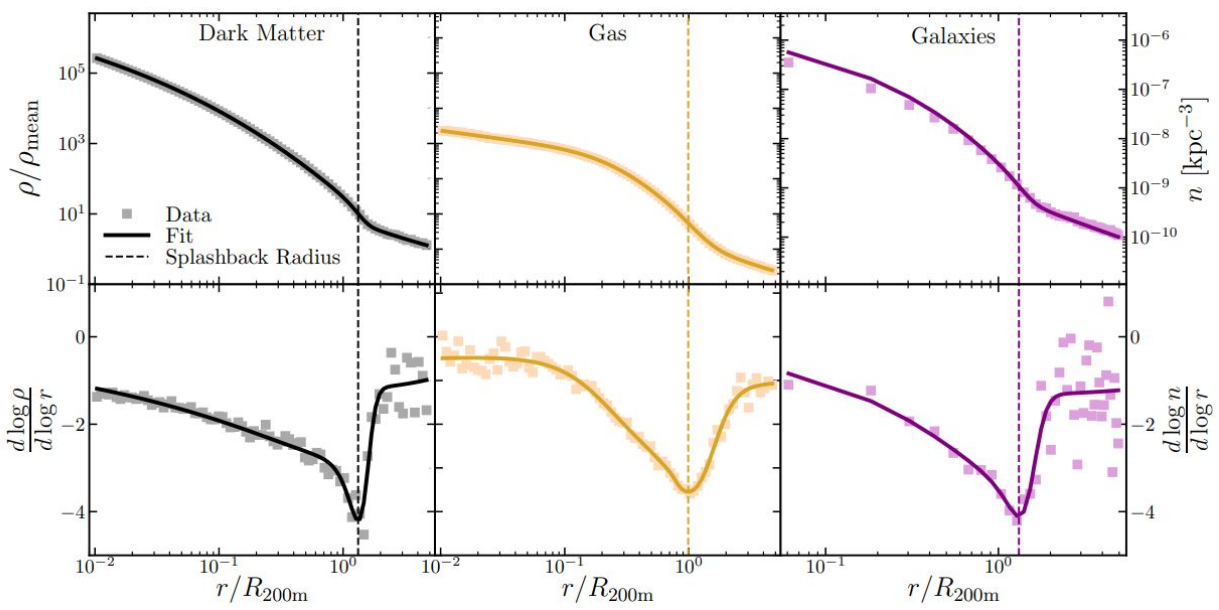
\includegraphics[width=0.6\textwidth]{assets/splashback.png}
    \caption{DM, gas and galaxy density profiles and splashback radius from TNG hydrosimulations \cite{ONeil2020}.}
\end{figure}

\section{The Intracluster Medium} \label{sec:icm}

\subsection{General Properties} \label{subsec:icm_general}

\begin{minipage}{0.56\textwidth}
The \bfit{intracluster medium} (ICM) is a hot ($T \sim 10^7$-$10^8\,\text{K}$), optically thin plasma that permeates the space between galaxies within a cluster. It is the product of gas infall into the deep gravitational potential well of the cluster's dark matter halo, heated primarily by accretion shocks and adiabatic compression during the hierarchical assembly of the structure. Once heated, the ICM is prevented from cooling efficiently at the cluster centre by two competing processes: feedback from the central AGN, and the sloshing of the plasma induced by mergers with infalling subclusters (a competition examined further in \cref{sec:cool_core}).
\end{minipage}%
\hfill
\begin{minipage}{0.4\textwidth}
    \centering
    \todo{Composite optical/millimetre image of the intracluster medium surrounding the Spiderweb Galaxy, hot gas detected with ALMA overlaid on an HST optical image (ESO/Di Mascolo et al.; HST: H. Ford).}
\end{minipage}

\medskip

Because clusters are the largest gravitationally bound structures to have formed via hierarchical assembly, the ICM also acts as a \textbf{fossil record} of cosmic chemical enrichment: the deep potential wells of clusters lock in place the metals synthesised and ejected by member galaxies over cosmic time, rather than allowing them to escape into the wider intergalactic medium.

\smallskip

The ICM is a fully ionised plasma, composed predominantly of hydrogen and helium with trace amounts of heavier, metallic elements (Fe, O, Ne, Si), at densities of order $n \sim 10^{-3}$-$10^{-1}\,\text{cm}^{-3}$, orders of magnitude more diffuse than any laboratory plasma. It is threaded by a weak but pervasive magnetic field, $B \sim 0.1$-$10\,\mu\text{G}$, varying on scales of $0.1$-$10\,\text{kpc}$, which is dynamically unimportant for the overall gas pressure but nonetheless influences the transport of charged particles and cosmic rays within the cluster.

\subsection{X-ray Emission and Spectrum} \label{subsec:icm_spectrum}

The ICM radiates predominantly in X-rays, through three distinct emission processes: \textbf{free-free} emission (thermal bremsstrahlung), which dominates and accounts for roughly $90\%$ of the total luminosity, appearing as a smooth continuum; \textbf{free-bound} emission, arising from the recombination of free electrons onto ions, also contributing to the continuum; and \textbf{bound-bound} emission, produced by the de-excitation of bound electrons and giving rise to discrete spectral lines.

\medskip

The bremsstrahlung X-ray emissivity, the luminosity radiated per unit volume and frequency, takes the form
$$
\epsilon_\nu \equiv \frac{dL}{dV\,d\nu} \propto n_e^2\, g(\nu,T)\, T^{-1/2}\, \exp\!\left(-\frac{h\nu}{k_B T}\right) ,
$$
where $g(\nu,T)$ is a slowly varying Gaunt factor. Three features of this expression are of direct diagnostic value. First, the emissivity scales as the square of the electron density, making X-ray emission an extremely sensitive tracer of the densest regions of the ICM. Second, the overall normalisation scales as $T^{-1/2}$. Third, and most importantly, the spectrum exhibits an exponential cut-off set by the electron's thermal kinetic energy, $k_B T$: the location of this cut-off directly encodes the ICM temperature, providing one of the primary means of measuring it observationally.

\medskip

\begin{minipage}{0.58\textwidth}
The observed ICM spectrum is not a pure bremsstrahlung continuum, but a superposition of the continuum with recombination and line features. At lower temperatures, recombination produces characteristic "edges" in the spectrum (for instance, a feature near $0.5$-$1\,\text{keV}$); above ${\sim}\,6\,\text{keV}$ the electron-capture cross-section drops sharply and these edges are smeared out. Superposed emission lines carry the signature of metal enrichment: soft X-ray lines ($0.5$-$2\,\text{keV}$) from elements such as O, Ne, and Mg appear only when these metals are not yet fully ionised (below ${\sim}\,6\,\text{keV}$), while the \bfit{Iron L-shell complex} near $1\,\text{keV}$ arises from hundreds of overlapping transitions in partially ionised iron ions (Fe$^{16+}$ to Fe$^{23+}$). The single most prominent tracer of metal enrichment, however, is the \bfit{Fe K-$\alpha$ complex} at $6.7\,\text{keV}$: since it remains the only accessible line at high redshift, it provides the sole means of determining a cluster's redshift directly from its X-ray spectrum.
\end{minipage}%
\hfill
\begin{minipage}{0.38\textwidth}
    \centering
    \todo{Bremsstrahlung X-ray spectra for hot gas at temperatures from 1 to 10 keV, showing the exponential cut-off shifting to higher energy with increasing temperature.}
\end{minipage}

\begin{observationblock}[Spectral fitting]
In modern X-ray astronomy, using satellites such as \textbf{Chandra} or \textbf{XMM-Newton}, the spectral resolution is not always sufficient to resolve individual emission lines. Instead, observed spectra are fitted against tabulated plasma radiation codes, which incorporate all the known emission processes (bremsstrahlung, recombination, and line emission) as a function of temperature and metallicity, allowing these physical parameters to be recovered even when individual features remain blended.
\end{observationblock}

\subsection{Radial Profiles of the ICM} \label{subsec:icm_profiles}

Because clusters are extended, resolved X-ray sources, it is possible to map how the physical properties of the ICM, its temperature, metallicity, and density, vary as a function of cluster-centric radius. These radial profiles both test the underlying physics of cluster formation and reveal the diversity introduced by each cluster's individual merger history.

\subsubsection{Temperature Profile} \label{subsubsec:icm_temperature}

\begin{minipage}[t]{0.62\textwidth}
Fitting the X-ray spectra measured in concentric radial annuli, after convolving the tabulated plasma emission models with the instrument response, yields the three-dimensional temperature profile of the ICM. At large radii, $R \gtrsim 0.2\,R_{200}$, the normalised temperature profile is found to be remarkably \bfit{self-similar} across the cluster population, a signature that the same gravity-driven physics of accretion and shock heating shapes the outskirts of all clusters in a common way.

\smallskip

Closer to the centre, however, clusters diverge into two distinct behaviours: some show a pronounced drop in temperature toward the core, the signature of \bfit{Cool-Core} (CC) clusters, while others exhibit an approximately flat central profile, characteristic of \bfit{Non-Cool-Core} (NCC) systems (a distinction explored further in \cref{sec:cool_core}). To accommodate this diversity within a single parametric description, Vikhlinin et al. (2006) introduced the model
$$
T_{3D}(r) = T_0\,\frac{(r/r_t)^{-a}}{\left[1+(r/r_t)^b\right]^{c/b}}\,\frac{x + T_{\min}/T_0}{x+1} ,
$$
whose flexible functional form can reproduce both the declining cores of CC clusters and the flatter profiles of NCC systems.
\end{minipage}%
\hfill
\begin{minipage}[t]{0.33\textwidth}
    \centering
    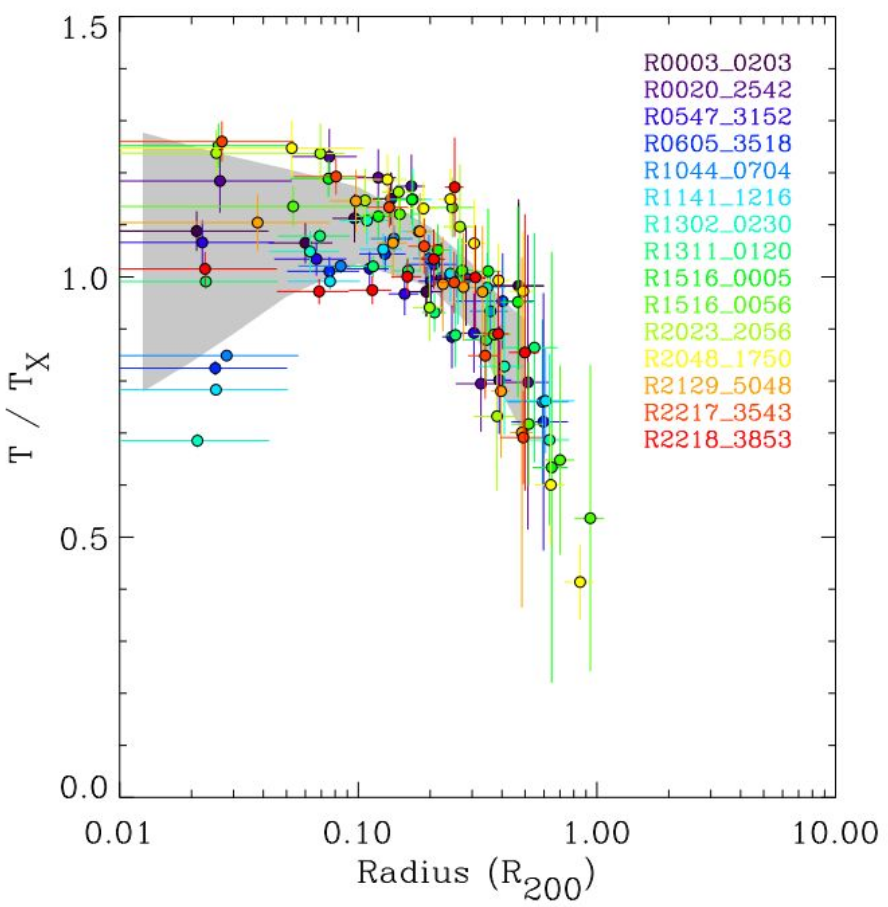
\includegraphics[width=\textwidth]{assets/gc-temp.png}
    \captionof{figure}{Temperature profile from XMM-Newton observations \cite{Pratt2006}.}
\end{minipage}

\subsubsection{Metallicity Profile} \label{subsubsec:icm_metallicity}

The radial metallicity profile of the ICM shows a sharp rise toward the cluster centre ($R/R_{500} \lesssim 0.2$), reaching approximately solar abundance in the innermost core; this central peak is driven by the ongoing metal production and enrichment from the central galaxy. At larger radii ($R/R_{500} \gtrsim 0.3$), the profile flattens to a remarkably constant value, $A \sim 0.3\,\text{solar}$. The consistency of this floor value across different clusters, together with the very large radii over which it extends, points to an early, widespread enrichment of the ICM, thought to have occurred around $z \sim 2$-$3$, well before the bulk of the cluster's present-day mass assembled. Measurements of the Fe abundance as a function of redshift independently corroborate this picture of early enrichment.

\smallskip

\begin{minipage}{0.55\textwidth}
The scatter observed in the metallicity profile at fixed radius is not random, but is closely tied to a cluster's dynamical state: \textbf{relaxed} systems display, on average, a higher central metallicity than \textbf{disturbed} ones, whose central abundance, while still enhanced relative to the outskirts, remains systematically lower. This pattern is consistent with a picture in which cluster mergers stir and mix the metal distribution through large-scale gas motions, diluting the sharp central enrichment that can otherwise build up undisturbed over a relaxed cluster's lifetime.
\end{minipage}%
\hfill
\begin{minipage}{0.4\textwidth}
    \centering
    \todo{Mean metallicity profile from a sample of ${\sim}200$ nearby galaxy groups and clusters observed with XMM-Newton, split into relaxed and disturbed subsamples, from Lovisari \& Reiprich (2019).}
\end{minipage}

\subsubsection{Gas Density Profile} \label{subsubsec:icm_density}

The simplest and most widely used description of the ICM density profile is the \bfit{$\beta$-model}. Assuming the gas is an isothermal sphere in hydrostatic equilibrium, the mass profile can be estimated in two equivalent ways: from the velocity dispersion of a collisionless tracer via the Jeans equation, or from the gas pressure and density directly,
$$
M(r) = -\frac{\sigma_r^2\,r}{G}\left[\frac{d\ln\rho}{d\ln r}\right]
\qquad\text{and}\qquad
M(r) = -\frac{kT\,r}{G\,\mu m_p}\left[\frac{d\ln\rho_g}{d\ln r}\right] .
$$
Equating these two mass estimates, under the assumption that the gas density profile traces the total (dark-matter-dominated) mass profile, motivates the definition of the dimensionless parameter
$$
\beta \equiv \frac{\sigma_r^2\,\mu m_p}{kT} ,
$$
which relates the specific kinetic energy of the collisionless matter to the thermal energy of the gas. If both the total matter distribution and the gas distribution follow the profile of a singular isothermal sphere truncated at a core radius $r_c$,
$$
\rho(r) = \rho_0\left(1+\left(\frac{r}{r_c}\right)^2\right)^{-3/2} ,
$$
then the gas density obeys the analogous relation
$$
\rho_g(r) = \rho_{g0}\left(1+\left(\frac{r}{r_c}\right)^2\right)^{-3\beta/2} .
$$
Fits to observed clusters typically recover $\beta \sim 2/3$, and the model provides an adequate description of relaxed systems (such as the Coma cluster) out to large radii; however, it performs poorly for dynamically disturbed clusters, whose density profiles are shaped by their individual merger and feedback history rather than by a single self-similar form.

\medskip

To accommodate this diversity, Vikhlinin et al. (2006) introduced a more flexible parametric model for the emission-measure profile ($n_p n_e \propto n_e^2$),
$$
n_p n_e = n_0^2\,\frac{(r/r_c)^{-\alpha}}{\left(1+r^2/r_c^2\right)^{3\beta - \alpha/2}}\,\frac{1}{\left(1+r^\gamma/r_s^\gamma\right)^{\epsilon/\gamma}} \;+\; \frac{n_{02}^2}{\left(1+r^2/r_{c2}^2\right)^{3\beta_2}} ,
$$
in which the first term describes the cluster outskirts and the second, independent term accounts for the central core, allowing the model to capture both the self-similar behaviour at large radii and the wide variety of central morphologies (cool cores, cavities, and disturbed cores) seen across the cluster population.

\subsubsection{Surface Brightness Profile} \label{subsubsec:icm_sb}

\begin{minipage}{0.56\textwidth}
Because the ICM is optically thin, the observed X-ray \textbf{surface brightness} at projected radius $R$ is simply the line-of-sight integral of the gas emissivity,
$$
S_x(R) = \frac{2}{4\pi}\int_R^\infty n_e^2\,\widetilde\Lambda(T)\,dz ,
$$
where $\widetilde\Lambda(T)$ is the temperature-dependent cooling function. Adopting a $\beta$-model for the underlying gas density profile, this integral can be evaluated analytically,
$$
S_x(R) = \frac{n_{e0}^2\,\widetilde\Lambda(T)\,r_c}{4\pi}\,\frac{\Gamma(0.5)\,\Gamma(3\beta - 0.5)}{\Gamma(3\beta)}\left(1+\left(\frac{R}{r_c}\right)^2\right)^{-3\beta+1/2}(1+z)^{-4} .
$$
Two features of this result have important observational consequences. Because $S_x \propto n_e^2$, the surface brightness falls steeply with radius, making the low-density cluster outskirts intrinsically difficult to observe. Because $S_x \propto (1+z)^{-4}$, the same cosmological surface-brightness dimming that dims extended sources at any wavelength makes it correspondingly difficult to obtain high signal-to-noise X-ray observations of clusters at high redshift: reaching a cluster at $z \simeq 1.4$ can require an exposure roughly twice as long as reaching one at $z \simeq 1.3$, and this cost grows rapidly with redshift.
\end{minipage}%
\hfill
\begin{minipage}{0.4\textwidth}
    \centering
    \todo{Chandra images of two clusters at similar mass but different redshift (z~0.26 and z~1), illustrating the dramatic surface-brightness dimming of the higher-redshift system.}
\end{minipage}

\section{X-ray Observations of Galaxy Clusters} \label{sec:icm_xray_obs}

\subsection{X-ray Telescopes: Chandra and XMM-Newton} \label{subsec:icm_telescopes}

The bulk of our knowledge of cluster X-ray emission derives from two flagship observatories, whose complementary designs (introduced in \cref{subsec:xray_optics,subsec:xray_detectors}) make them suited to different aspects of cluster science.

\smallskip

\subsubsection{Chandra}

\textbf{Chandra} (NASA), operating from 0.5 to 9\,keV over a field of view of ${\sim}\,16\,\text{arcmin}$, delivers an exceptional angular resolution of ${\sim}\,0.5''$, achieved through its Advanced CCD Imaging Spectrometer (ACIS), an array of CCD chips arranged into an imaging (ACIS-I) and a spectroscopic (ACIS-S) configuration. This superb resolution makes Chandra the instrument of choice for resolving fine substructure within a cluster, such as cold fronts, shock edges, and filamentary features associated with mergers and AGN-driven cavities.

\subsubsection{XMM-Newton}

\textbf{XMM-Newton} (ESA), covering 0.3 to 10\,keV over a wider field of view of ${\sim}\,30\,\text{arcmin}$, trades some angular resolution (${\sim}\,6''$) for substantially higher collecting area and throughput. Its European Photon Imaging Camera (EPIC) combines two types of CCD detector: the Metal-Oxide-Semiconductor (MOS) cameras, each comprising 7 CCDs, and the PN-CCD camera, comprising 12 CCDs. The resulting higher sensitivity makes XMM-Newton particularly well suited to mapping the faint, diffuse emission of cluster outskirts, complementing Chandra's strength in resolving compact central structure.

\begin{observationblock}[Chandra versus XMM-Newton]
The two observatories are frequently used in tandem for the same targets, since their strengths are complementary rather than redundant: Chandra's superior angular resolution reveals substructures such as filaments and sharp edges that XMM-Newton's coarser point-spread function smooths over, while XMM-Newton's larger effective area and field of view make it markedly more sensitive to the low surface brightness emission of cluster outskirts, which Chandra's smaller collecting area struggles to detect at comparable exposure times.
\end{observationblock}

\subsection{Event Files, Background, and Source Detection} \label{subsec:icm_background}

X-ray observations are delivered not as conventional images but as \bfit{event files}: a list of individually detected photons, each tagged with its arrival time, detector position, and pulse-height (energy) channel. Because each incoming X-ray photon liberates many electron-hole pairs in the CCD (in contrast to the single electron produced by an optical photon), these detectors function simultaneously as imagers and as photon-counting spectrometers, recording both where and at what energy each photon arrived.

\medskip

Any X-ray observation is contaminated by a \textbf{background} with both astrophysical and instrumental origins. The astrophysical component comprises diffuse emission from the Milky Way itself, principally the Local Hot Bubble and the hot gas of the Galactic halo, typically modelled as a combination of two thermal components, together with the cumulative emission of unresolved extragalactic point sources (predominantly background AGN), modelled as an absorbed power law. The instrumental component arises from the telescope structure itself being struck by high-energy charged particles, whose interactions with the detector are registered indistinguishably from genuine X-ray photons.

\medskip

\begin{minipage}{0.6\textwidth}
Extracting a clean measurement of the cluster's own emission from this combination of source and background requires a multi-step \bfit{source detection} procedure. First, all individually resolved point sources in the field, chiefly foreground stars and background AGN unrelated to the cluster, are identified and masked. The astrophysical and instrumental background components are then characterised and subtracted from the remaining, diffuse emission. Only after this cleaning step does the smooth, extended emission of the cluster itself emerge clearly, ready for the radial profile analysis described in \cref{subsec:icm_profiles}.
\end{minipage}%
\hfill
\begin{minipage}{0.35\textwidth}
    \centering
    \todo{Four-panel sequence: raw Chandra field, detected point sources circled and masked, background-subtracted image, and final cleaned cluster detection.}
\end{minipage}

\medskip

In practice, deriving the density and temperature profiles of \cref{subsec:icm_profiles} proceeds by measuring the mean surface brightness and the mean spectrum within a series of concentric radial annuli or bins, and then fitting each of these binned measurements independently: the surface brightness profile is fit to recover the gas density profile (\cref{subsubsec:icm_density,subsubsec:icm_sb}), while the spectrum extracted in each bin is fit to recover the local temperature (\cref{subsubsec:icm_temperature}).

\section{Cluster Masses from X-ray Observations} \label{sec:icm_masses}

\subsection{Hydrostatic Mass Estimates} \label{subsec:hse}

\begin{minipage}{0.58\textwidth}
For a system in \bfit{hydrostatic equilibrium}, the inward pull of gravity is everywhere balanced by the outward gradient of the gas pressure,
$$
\nabla P_{\text{gas}} = -\rho_{\text{gas}}\,\nabla\Phi .
$$
Assuming spherical symmetry, this reduces to
$$
\frac{dP}{dr} = -\rho_{\text{gas}}\,\frac{d\Phi}{dr} = -\rho_{\text{gas}}\,\frac{GM(r)}{r^2} .
$$
Combining this with the ideal gas equation of state, $P = n k_B T$, allows the total gravitating mass enclosed within radius $r$, dark matter included, to be estimated directly from the observed gas density and temperature profiles:
$$
M(r) = -\frac{r^2}{\rho_{\text{gas}}}\frac{dP}{dr} = -\frac{r}{G}\frac{kT}{\mu m_p}\left[\frac{d\ln\rho_{\text{gas}}}{d\ln r} + \frac{d\ln T}{d\ln r}\right] .
$$
This \bfit{hydrostatic mass} estimate is one of the principal routes by which X-ray observations constrain cluster masses, and, by extension, cosmological parameters sensitive to the cluster mass function.
\end{minipage}%
\hfill
\begin{minipage}{0.38\textwidth}
    \centering
    \todo{Schematic of a spherical gas cloud in hydrostatic equilibrium, with inward gravity arrows balanced by outward gas-pressure arrows.}
\end{minipage}

\medskip

The derivation rests on two simplifying assumptions: hydrostatic equilibrium itself, meaning that non-thermal pressure support is negligible, and spherical symmetry. Both assumptions are reasonably well satisfied in dynamically \textbf{relaxed} clusters. In \textbf{disturbed}, merging systems, however, turbulent gas motions inject an additional, non-thermal pressure support, governed by the Euler equation
$$
\frac{\partial \mathbf{v}}{\partial t} + (\mathbf{v}\cdot\nabla)\mathbf{v} = -\frac{1}{\rho_{\text{gas}}}\nabla P_{\text{gas}} - \nabla\phi ,
$$
which is entirely neglected by the simple hydrostatic mass formula above. Recent high-resolution spectroscopy (e.g.\ with XRISM) has begun to measure this non-thermal pressure fraction directly, finding it to increase from a few percent in the core to several percent near $R_{2500}$ in relaxed systems such as Abell 2029.

\subsection{The Hydrostatic Mass Bias} \label{subsec:hse_bias}

\begin{minipage}{0.55\textwidth}
Because the simple hydrostatic mass estimate neglects any non-thermal pressure support, it systematically \textbf{underestimates} the true cluster mass whenever such support is present, an effect known as the \bfit{hydrostatic mass bias}. Comparisons between hydrostatic mass estimates and the true mass in cosmological simulations, where the true mass is known exactly, indicate a typical bias of order $10$-$20\%$, with the effect being markedly stronger for dynamically disturbed clusters than for relaxed ones: mock observations of clusters spanning a range of dynamical states consistently recover mass profiles for disturbed systems that lie below those of relaxed systems at the same true mass.
\end{minipage}%
\hfill
\begin{minipage}{0.42\textwidth}
    \centering
    \todo{Scaled hydrostatic mass profiles for 75 simulated massive clusters, showing disturbed systems (red) lying systematically below relaxed systems (blue) at fixed radius; adapted from Bartalucci et al. 2019.}
\end{minipage}

\medskip

A further, more subtle source of uncertainty in the derived radial profiles comes from the choice of \textbf{cluster centre}. Two common definitions, the X-ray surface-brightness peak and the X-ray centroid, generally agree closely for relaxed, symmetric clusters, but can diverge substantially in disturbed systems whose X-ray morphology is elongated or multiply peaked, introducing an additional, dynamical-state-dependent systematic into the mass estimate.

\section{Cool-Core and Non-Cool-Core Clusters} \label{sec:cool_core}

Building on the temperature profile diversity introduced in \cref{subsubsec:icm_temperature}, \bfit{Cool-Core} (CC) and \bfit{Non-Cool-Core} (NCC) clusters exhibit distinct, physically linked signatures across their density, temperature, and metallicity profiles. Cool-core clusters show an elevated central gas density, which drives efficient radiative cooling; a temperature that drops sharply toward the centre, indicating that the gas is losing energy faster than it can be replenished; and a strong central enhancement in metallicity, reflecting the undisturbed accumulation of metals produced by the central galaxy over a long, quiescent period. Non-cool-core clusters lack all three signatures, instead showing a flatter, hotter, and more chemically uniform central distribution.

\smallskip

These two classes map directly onto the dynamical history of the cluster. Cool cores are found in \textbf{relaxed} systems that have not experienced a major merger for several billion years, allowing their dense central gas to cool and their metal content to accumulate undisturbed. Non-cool cores, conversely, characterise \textbf{disturbed} systems that have recently undergone a major merger: the immense kinetic energy of the collision drives shocks and turbulence that stir the gas, injecting heat and erasing any pre-existing cool core, in the same way that mergers dilute the central metallicity peak discussed in \cref{subsubsec:icm_metallicity}.

\begin{tipsblock}[The cooling flow problem]
Based purely on X-ray observations of its density and temperature, the dense central gas of a cool-core cluster should radiate away its energy efficiently and cool rapidly to very low temperatures ($T < 10^4\,\text{K}$), producing a massive \bfit{cooling flow} of gas onto the central galaxy at rates of order $100$-$1000\,M_\odot\,\text{yr}^{-1}$. In practice, however, X-ray spectroscopy shows that while the gas does cool toward the centre, it never drops below a characteristic floor temperature of order $T \sim 10^7\,\text{K}$: the large reservoirs of cold gas and correspondingly high star formation rates predicted by simple cooling-flow models are largely absent, with the observed cooling rate falling roughly a factor of five below the naive prediction.

\smallskip

The leading resolution to this "cooling flow problem" is that the gas is continuously reheated, most plausibly by feedback from the central supermassive black hole's active nucleus (\cref{ch:agn}): jets and outflows from the AGN inject just enough mechanical energy back into the surrounding gas to balance radiative losses, holding the cool core in a state of rough thermal equilibrium rather than allowing it to collapse.
\end{tipsblock}

\smallskip

Finally, because the X-ray surface brightness scales as $n_e^2$ (\cref{subsubsec:icm_sb}), the denser cores of cool-core clusters render them systematically easier to detect in flux-limited X-ray surveys than their non-cool-core counterparts. This \textbf{selection effect} must be carefully modelled in any cosmological analysis that relies on X-ray-selected cluster catalogues, since an uncorrected excess of cool cores in a survey would otherwise bias the inferred cluster mass function and the cosmological parameters derived from it.

\section{Future Facilities: Athena} \label{sec:athena}

\begin{minipage}{0.55\textwidth}
The \textbf{Advanced Telescope for High-Energy Astrophysics} (Athena, ESA) is a next-generation X-ray observatory designed to combine a substantially larger effective area and field of view with the high spectral resolution of a micro-calorimeter instrument (the X-ray Integral Field Unit, X-IFU), analogous in principle to the instrument flown on Astro-H/XRISM (\cref{subsubsec:cmb_history}). Simulated observations of deep survey fields indicate that Athena will detect a comparable or greater number of sources than Chandra over a much wider field of view, using only a small fraction of the exposure time, dramatically improving the efficiency of wide-area, high-redshift cluster surveys.
\end{minipage}%
\hfill
\begin{minipage}{0.4\textwidth}
    \centering
    \todo{Simulated Athena X-IFU spectrum of a cluster compared to XMM-Newton/pn, XRISM/SXS, and Chandra/ACIS-I, showing individually resolved metal lines (O, Ne, Mg, Si, S, Fe) at far higher signal-to-noise than current instruments.}
\end{minipage}

\medskip

By resolving individual metal emission lines with high statistical precision across large cluster samples, Athena's X-IFU is expected to transform measurements of the ICM's metallicity and temperature structure described in \cref{subsec:icm_profiles}, extending detailed profile studies to higher redshift and lower mass than is currently feasible, and providing a far more direct probe of the chemical enrichment history encoded in the ICM.                        